\documentclass[]{article}

\title{Homework 4}
\author{Kelsey Iafrate}
\usepackage{geometry}

\geometry{margin=1in}

\usepackage{Sweave}
\begin{document}

\maketitle

\Sconcordance{concordance:Homework4.tex:Homework4.Rnw:%
1 8 1 1 0 14 1 1 2 1 0 4 1 10 0 1 2 4 1 1 2 25 0 1 2 8 1 1 2 1 0 1 1 20 %
0 2 1 23 0 1 2 8 1 1 2 1 0 1 1 7 0 1 2 4 1 1 2 8 0 1 2 10 1 1 2 1 0 1 1 %
2 2 1 1 10 0 1 2 6 1 1 2 26 0 1 2 7 1 1 2 41 0 1 2 1 1 27 0 1 2 4 0 1 3 %
4 1 1 2 24 0 1 2 10 1 1 3 2 0 1 1 7 0 1 2 8 1}


\begin{enumerate}

\item

\begin{enumerate}

\item


\begin{Schunk}
\begin{Sinput}
> VACATION <- read.csv("~/Documents/Stat103/Data Sets/VACATION.csv")
> attach(VACATION)
> model <- lm(Price~Lot.size+Trees+Distance)
> plot.lm(model, which = 1)
> shapiro.test(model$residuals)
\end{Sinput}
\begin{Soutput}
	Shapiro-Wilk normality test

data:  model$residuals
W = 0.9688, p-value = 0.1271
\end{Soutput}
\end{Schunk}
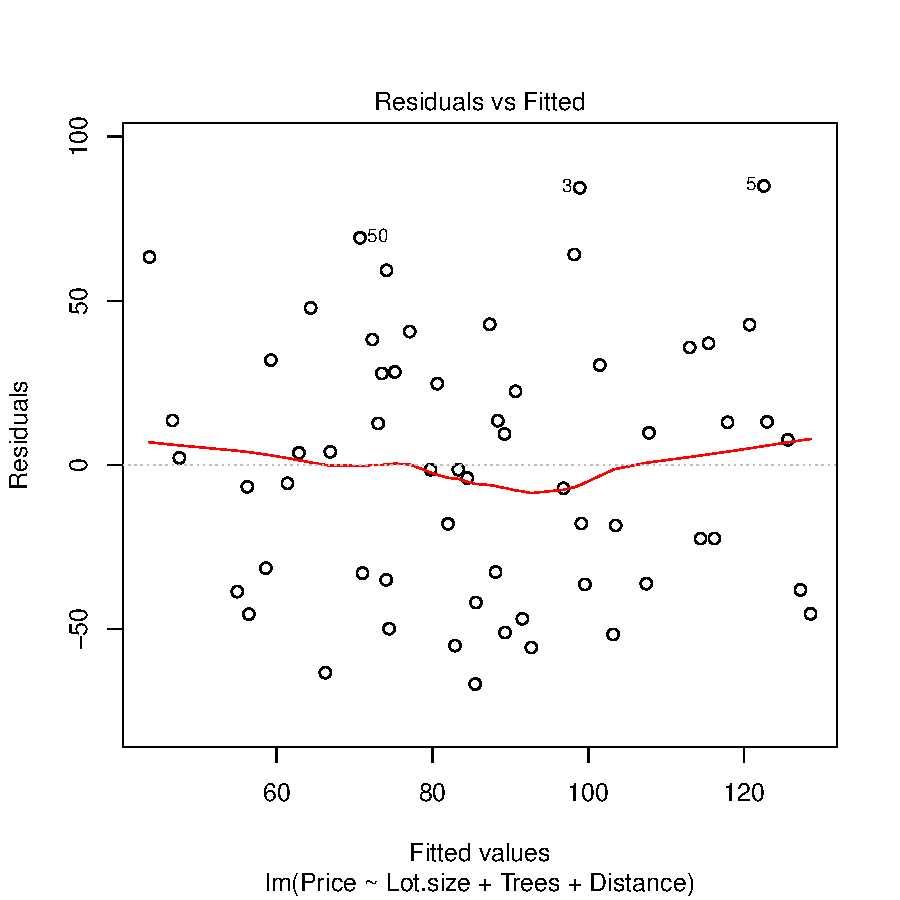
\includegraphics{Homework4-001}

There does not appear to be a significant curve in the residuals, so the variance appears to be constant. The Shapiro-Wilk test outputs a p-value of ~0.1, so we can not reject that the residuals are normally distributed. Therefore, the model assumptions appear to be satisfied. 

\item

\begin{Schunk}
\begin{Sinput}
> summary(model)
\end{Sinput}
\begin{Soutput}
Call:
lm(formula = Price ~ Lot.size + Trees + Distance)

Residuals:
    Min      1Q  Median      3Q     Max 
-66.702 -35.272   0.365  28.854  84.966 

Coefficients:
            Estimate Std. Error t value Pr(>|t|)   
(Intercept)  51.3912    23.5165   2.185   0.0331 * 
Lot.size      0.6999     0.5589   1.252   0.2156   
Trees         0.6788     0.2293   2.960   0.0045 **
Distance     -0.3784     0.1952  -1.938   0.0577 . 
---
Signif. codes:  0 ‘***’ 0.001 ‘**’ 0.01 ‘*’ 0.05 ‘.’ 0.1 ‘ ’ 1

Residual standard error: 40.24 on 56 degrees of freedom
Multiple R-squared:  0.2425,	Adjusted R-squared:  0.2019 
F-statistic: 5.975 on 3 and 56 DF,  p-value: 0.001315
\end{Soutput}
\end{Schunk}

The multiple R-squared is 24.25\% and the adjested R-squared is 20.19\%. This tells us that the variation in house price is not very well explained by the model. Only 20.19\% of the variation in house price can be explained by this original model

\item

The number of mature trees is definitely linearly related to the price of the house with a p-value of 0.0045. A house's distance from the lake is somewhat linearly related to the price since it has a p-value of 0.0577. We cannot conclude that lot size is linearly related to the house price. 

\item

\begin{Schunk}
\begin{Sinput}
> library(MASS)
> step <- stepAIC(model, way='both')
\end{Sinput}
\begin{Soutput}
Start:  AIC=447.25
Price ~ Lot.size + Trees + Distance

           Df Sum of Sq    RSS    AIC
- Lot.size  1    2540.2  93235 446.91
<none>                   90694 447.25
- Distance  1    6082.5  96777 449.15
- Trees     1   14192.6 104887 453.98

Step:  AIC=446.91
Price ~ Trees + Distance

           Df Sum of Sq    RSS    AIC
<none>                   93235 446.91
- Distance  1    8366.9 101601 450.07
- Trees     1   20011.3 113246 456.58
\end{Soutput}
\begin{Sinput}
> newModel <- lm(Price~Trees+Distance)
> summary(newModel)         
\end{Sinput}
\begin{Soutput}
Call:
lm(formula = Price ~ Trees + Distance)

Residuals:
    Min      1Q  Median      3Q     Max 
-73.600 -33.159  -4.829  33.828  97.281 

Coefficients:
            Estimate Std. Error t value Pr(>|t|)    
(Intercept)  75.5248    13.5464   5.575 7.06e-07 ***
Trees         0.7671     0.2193   3.498 0.000917 ***
Distance     -0.4327     0.1913  -2.262 0.027549 *  
---
Signif. codes:  0 ‘***’ 0.001 ‘**’ 0.01 ‘*’ 0.05 ‘.’ 0.1 ‘ ’ 1

Residual standard error: 40.44 on 57 degrees of freedom
Multiple R-squared:  0.2213,	Adjusted R-squared:  0.1939 
F-statistic: 8.097 on 2 and 57 DF,  p-value: 0.0008031
\end{Soutput}
\end{Schunk}

The stepAIC function determined that removing only lot size gave a better model. 

\item

The average price of homes of equal distance from the lake will increase by \$767 for every additional mature tree on the lot. The average price of a home with a fixed number of mature trees on the lot will decrease on average by \$433 for every foot farther it is away from the lake.

\item

\begin{Schunk}
\begin{Sinput}
> newData <- data.frame("Lot.size" = 40,"Trees" = 50, "Distance" = 75)
> predict(model, newData,interval = "prediction")
\end{Sinput}
\begin{Soutput}
       fit      lwr     upr
1 84.95099 2.794942 167.107
\end{Soutput}
\end{Schunk}

We predict with 95\% confidence a 40,000 square foot house with 50 mature trees that is 75 feet from the lake to sell for between \$2,795 and \$167,107.

\item

\begin{Schunk}
\begin{Sinput}
> predict(model, newData,interval = "confidence")
\end{Sinput}
\begin{Soutput}
       fit      lwr      upr
1 84.95099 69.12573 100.7762
\end{Soutput}
\end{Schunk}

We are 95\% confident that on average 40000 square foot houses with 50 mature trees that are 75 feet from the lake will sell for between \$69,126 and \$100,776.

\end{enumerate}

\item

\begin{enumerate}

\item

\begin{Schunk}
\begin{Sinput}
> DRYWALL <- read.csv('~/Documents/Stat103/Data Sets/DRYWALL.csv')
> attach(DRYWALL)
> model <- lm(Drywall~Permits+Mortgage+A.Vacancy+O.Vacancy)
> plot.lm(model, which = 1)
> shapiro.test(model$residuals)
\end{Sinput}
\begin{Soutput}
	Shapiro-Wilk normality test

data:  model$residuals
W = 0.9684, p-value = 0.6267
\end{Soutput}
\end{Schunk}
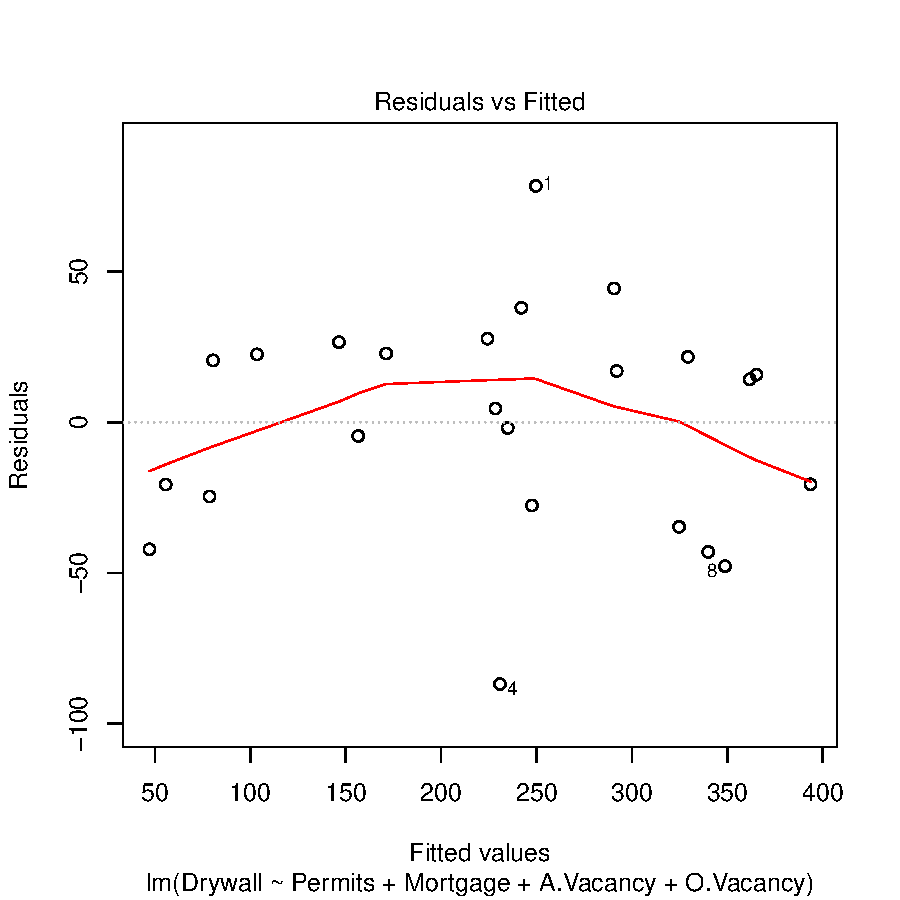
\includegraphics{Homework4-006}

There appears to be a curve in the residuals, which implies the variance may not be constant. However, the curve does not deviate away from zero too much, so I will choose to accept the assumption that the residual variance is constant.

The Shapiro-Wilk test determines that we cannot reject that the residuals are normally distributed, so this assumption is satisfied.

\item

\begin{Schunk}
\begin{Sinput}
> summary(model)
\end{Sinput}
\begin{Soutput}
Call:
lm(formula = Drywall ~ Permits + Mortgage + A.Vacancy + O.Vacancy)

Residuals:
    Min      1Q  Median      3Q     Max 
-86.822 -25.351   9.409  22.602  78.391 

Coefficients:
            Estimate Std. Error t value Pr(>|t|)    
(Intercept) -111.828    134.343  -0.832    0.416    
Permits        4.763      0.395  12.057 2.39e-10 ***
Mortgage      16.988     15.159   1.121    0.276    
A.Vacancy    -10.528      6.394  -1.646    0.116    
O.Vacancy      1.308      2.791   0.469    0.645    
---
Signif. codes:  0 ‘***’ 0.001 ‘**’ 0.01 ‘*’ 0.05 ‘.’ 0.1 ‘ ’ 1

Residual standard error: 40.13 on 19 degrees of freedom
Multiple R-squared:  0.8935,	Adjusted R-squared:  0.8711 
F-statistic: 39.86 on 4 and 19 DF,  p-value: 5.448e-09
\end{Soutput}
\end{Schunk}

The multiple R-squared is 89.35\%, and the adjusted R-squared, which is more appropriate for this model, is 87.11\%. This tells us that 87.11\% of the variation in the demand for dry wall can be explained by the model. This indicates the model will precicely predict the demand for drywall.

\item

The only explanatory variable that is linearly related to the demand for drywall is the number of building permits issued in this model.

\item
\begin{Schunk}
\begin{Sinput}
> stepAIC(model, direction="both")
\end{Sinput}
\begin{Soutput}
Start:  AIC=181.62
Drywall ~ Permits + Mortgage + A.Vacancy + O.Vacancy

            Df Sum of Sq    RSS    AIC
- O.Vacancy  1       354  30955 179.89
- Mortgage   1      2023  32624 181.15
<none>                    30602 181.62
- A.Vacancy  1      4366  34967 182.82
- Permits    1    234133 264734 231.40

Step:  AIC=179.89
Drywall ~ Permits + Mortgage + A.Vacancy

            Df Sum of Sq    RSS    AIC
- Mortgage   1      1973  32928 179.38
<none>                    30955 179.89
- A.Vacancy  1      4254  35210 180.99
+ O.Vacancy  1       354  30602 181.62
- Permits    1    234503 265459 229.47

Step:  AIC=179.38
Drywall ~ Permits + A.Vacancy

            Df Sum of Sq    RSS    AIC
<none>                    32928 179.38
+ Mortgage   1      1973  30955 179.89
- A.Vacancy  1      4494  37422 180.45
+ O.Vacancy  1       304  32624 181.15
- Permits    1    234445 267373 227.64

Call:
lm(formula = Drywall ~ Permits + A.Vacancy)

Coefficients:
(Intercept)      Permits    A.Vacancy  
     44.138        4.745      -10.660  
\end{Soutput}
\begin{Sinput}
> otherModel <- lm(Drywall~Permits)
> stepAIC(otherModel, scope = ~.+Mortgage+A.Vacancy+O.Vacancy, direction="forward")
\end{Sinput}
\begin{Soutput}
Start:  AIC=180.45
Drywall ~ Permits

            Df Sum of Sq   RSS    AIC
+ A.Vacancy  1    4494.0 32928 179.38
<none>                   37422 180.45
+ Mortgage   1    2212.4 35210 180.99
+ O.Vacancy  1     196.3 37226 182.32

Step:  AIC=179.38
Drywall ~ Permits + A.Vacancy

            Df Sum of Sq   RSS    AIC
<none>                   32928 179.38
+ Mortgage   1    1972.8 30955 179.89
+ O.Vacancy  1     303.6 32624 181.15

Call:
lm(formula = Drywall ~ Permits + A.Vacancy)

Coefficients:
(Intercept)      Permits    A.Vacancy  
     44.138        4.745      -10.660  
\end{Soutput}
\begin{Sinput}
> newModel <- lm(Drywall~Permits+A.Vacancy)
> 
\end{Sinput}
\end{Schunk}

The stepAIC function determined that the only two significant explanatory variables are the number of building permits sold and the apartment vacancy rate. Even here, the A.Vacancy rate has a very high p-value of 0.105. I did a foreward stepAIC analysis and got the same model. I also did an experiment where I did a foreward stepAIC without apartment vacancy to see if R was simply going to add another explanatory variable no matter what. It did not. I find it odd that R's default step function would add in an explanatory variable with such a high p-value. Is there an explanation for this?

\item

\begin{Schunk}
\begin{Sinput}
> summary(newModel)
\end{Sinput}
\begin{Soutput}
Call:
lm(formula = Drywall ~ Permits + A.Vacancy)

Residuals:
    Min      1Q  Median      3Q     Max 
-91.978 -25.940   7.148  25.743  83.123 

Coefficients:
            Estimate Std. Error t value Pr(>|t|)    
(Intercept)  44.1381    34.1777   1.291    0.211    
Permits       4.7450     0.3881  12.228 5.14e-11 ***
A.Vacancy   -10.6599     6.2967  -1.693    0.105    
---
Signif. codes:  0 ‘***’ 0.001 ‘**’ 0.01 ‘*’ 0.05 ‘.’ 0.1 ‘ ’ 1

Residual standard error: 39.6 on 21 degrees of freedom
Multiple R-squared:  0.8854,	Adjusted R-squared:  0.8745 
F-statistic: 81.14 on 2 and 21 DF,  p-value: 1.32e-10
\end{Soutput}
\end{Schunk}

The model predicts that with apartment vacancy held constant, sales of drywall will go up by 475 sheets on average for every additional building permit issued. The model predicts 1000 fewer sheets of dry wall will be sold on average for every percent raise in appartment vacancy while the number of permits being issued remains the same. 

\item

For the original multiple R-squared is 89.35\%, and the adjusted R-squared, which is more appropriate for this model, is 87.11\%.
For the new model multiple R-squared is 88.54\%, and the adjusted R-squared, which is more appropriate for this model, is 87.45\%.
Though the multiple R-squared went down for the new model compared to the original, we get a slight gain of .34\% in the adjusted R-squared for the new model.

\item

\begin{Schunk}
\begin{Sinput}
> newData <- data.frame("Permits" = 50, "Mortgage" = 8.5, "A.Vacancy" = 4.2, 
+                       "O.Vacancy" = 14)
> predict.lm(model,newData, interval = "prediction")
\end{Sinput}
\begin{Soutput}
       fit      lwr      upr
1 244.8221 156.3627 333.2815
\end{Soutput}
\end{Schunk}

Next month, if 50 building permits are given, the mortgage rate is 8.5\%, apartment vacancy is at 4.2\%, and office vacancy is at 14\%, we predict with 95\% confidence that between 15636 and 33328 sheets of dry wall will be sold.

\end{enumerate}


\end{enumerate}

\end{document}
